\newproblem*{oop}{%
  % This is an essay style question.
  Describe what is meant by object-oriented programming.%
}

\begin{defproblem}{inheritance}
  % This is an essay style question.
 Describe what is meant by the term \emph{inheritance} in
 object-oriented programming. Use examples.
\end{defproblem}

\begin{defproblem}{weightedcoin}%
  \begin{onlyproblem}
    A coin is weighted so that heads is four times as likely
    as tails. Find the probability that:
    \begin{textenum}
      \item tails appears,
      \item heads appears
    \end{textenum}%
  \end{onlyproblem}%
  \begin{onlysolution}
    Let $p=P(T)$, then $P(H)=4p$. We require $P(H)+P(T)=1$,
    so $4p+p=1$, hence $p=\frac{1}{5}$. Therefore:
    \begin{textenum}
      \item $P(T)=\frac{1}{5}$,
      \item $P(H)=\frac{4}{5}$
    \end{textenum}
  \end{onlysolution}
\end{defproblem}

\begin{defproblem}{validprobspaces}
\begin{onlyproblem}%
Under which of the following functions does
$S=\{a_1,a_2\}$ become a probability space?
\par
\begin{textenum}
\begin{tabular}{ll}
\item $P(a_1)=\frac{1}{3}$, $P(a_2)=\frac{1}{2}$
&
\item\label{validprobspacescorrect1} $P(a_1)=\frac{3}{4}$,
$P(a_2)=\frac{1}{4}$
\\
\item\label{validprobspacescorrect2} $P(a_1)=1$, $P(a_2)=0$
&
\item $P(a_1)=\frac{5}{4}$, $P(a_2)=-\frac{1}{4}$
\end{tabular}
\end{textenum}
\end{onlyproblem}%
\begin{onlysolution}%
\ref{validprobspacescorrect1} and \ref{validprobspacescorrect2}%
\end{onlysolution}
\end{defproblem}

\begin{defproblem}{digraph}
  % This problem requires the tikz package
  \begin{onlyproblem}\label{ex:digraph}
  Identify, if any, the sinks and sources of the digraph shown 
  in Figure~\ref{fig:digraph}. 

  \begin{figure}[tbh]
    \centering
      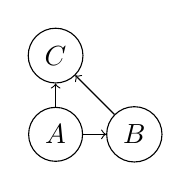
\begin{tikzpicture}[every node/.style={draw,circle}]
         \path (0,0) node (A) {$A$}
               (1,0) node (B) {$B$}
               (0,1) node (C) {$C$};
         \draw[->] (A) -- (B);
         \draw[->] (B) -- (C);
         \draw[->] (A) -- (C);
      \end{tikzpicture}
    \par
    \caption{Digraph for Question~\ref{ex:digraph}}
    \label{fig:digraph}
  \end{figure}
  \end{onlyproblem}
  \begin{onlysolution}
  $A$ is a source and $C$ is a sink.
  \end{onlysolution}
\end{defproblem}
